\documentclass{article}
\usepackage[utf8]{inputenc}
\usepackage[danish]{babel}
\usepackage{hyperref}
\usepackage{graphicx}
\usepackage{float}
\usepackage{listings}

\title{Sammenligning af NetLogo og Mesa}
\date{\today}

\begin{document}

\maketitle

\section{Oversigt}
\textit{Agent-baserede modeller} er modeller, som kan simulere interaktioner mellem flere forskellige, individuelle \textit{agenter} i et system, typisk med det formål at danne en forståelse for systemet som en helhed. Simulationerne viser typisk, hvordan systemet ændrer sig over tid, afhængigt af vilkårlige startparametre og agenternes opførsel.\\\\
Vi sammenligner to værktøjer, som tilbyder simulationer af agent-baserede modeller. Det ene er \textbf{NetLogo}\footnote{\url{ccl.northwestern.edu/netlogo}}, som er et selvstændigt miljø der benytter sit eget domænespecifikke sprog. Det andet er \textbf{Mesa}\footnote{\url{mesa.readthedocs.io/en/master/index.html}}, som er et framework til Python. Vi giver et overblik over hvert, og sammenligner deres fordele og ulemper.

\section{NetLogo}
NetLogo er et udviklingsmiljø til simulation af agent-baserede modeller. Miljøet tilbyder sit eget sprog (også kaldet \texttt{NetLogo}) til at opstille modellerne, samt et visuelt interface, som gør det muligt at simulere sin model og justere parametre hen ad vejen.\\\\
Sproget er forholdsvist nemt at læse og forstå. Mange af de mest nødvendige funktionaliteter eksisterer som indbyggede funktioner, så ens egen simple funktioner kan typisk holdes på under 10 linjer. Det kræves at man har forståelse for simple datatyper som integers, bools, strings etc., samt control-flow i form af if-sætninger. Løkker kan normalt undgås ved istedet at bruge \texttt{ask}-keywordet.
\begin{figure}[H]
  \begin{lstlisting}[frame=single]
    ask people [
      set shape "person"
      set is-immune false
      ifelse random-float 100 < 5
      [ infect ]
      [ cure ]
    ]
  \end{lstlisting}
  \caption{Kodeeksempel fra \texttt{epidemic.nlogo}.}
\end{figure}
NetLogo-miljøet tilbyder også en visuel interface, hvor det er muligt at se agenternes opførsel i realtid. Her kan man også tilføje bl.a. knapper og "sliders", der tillader en at justere parametre undervejs, eller små graf-vinduer, der viser udvalgte datapunkter.
\begin{figure}[H]
  \centering
  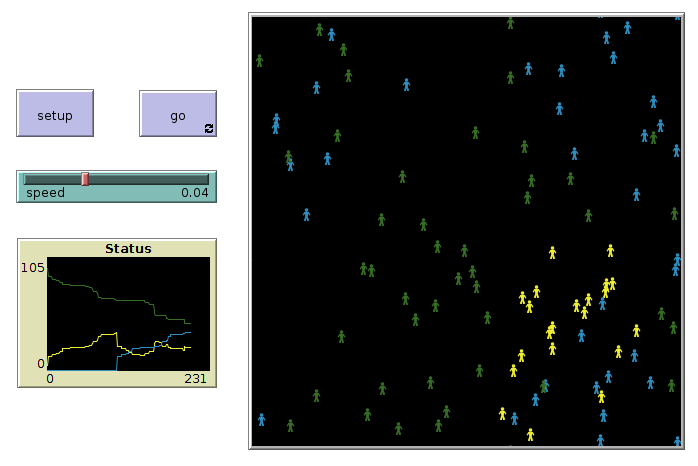
\includegraphics[width=0.75\textwidth]{epidemic_netlogo.png}
  \caption{Visuel interface fra \texttt{epidemic.nlogo}.}
\end{figure}
\section{Mesa}
Mesa er er framework til Python. Det implementerer et sæt af basis-klasser, herunder \texttt{Model} og \texttt{Agent}, som man så skal tilføje funktionalitet til. Dette kræver en god forståelse for klasser i Python, afhængigt af, hvor meget man vil lade eleverne implementere selv. For at visualisere modellen i realtid kræves desuden, at man implementerer et \texttt{VisualizationElement}, eller benytter en af de eksisterende, som f.eks. en gitter-visualisering med \texttt{CanvasGrid}. Hvis man ønsker en mere specifik model, skal man, ud over at implementere et \texttt{VisualizationElement}, også kode en del af det visuelle i JavaScript, da Mesa bruger en web-server til visuel præsentation.
\begin{figure}[H]
  \centering
  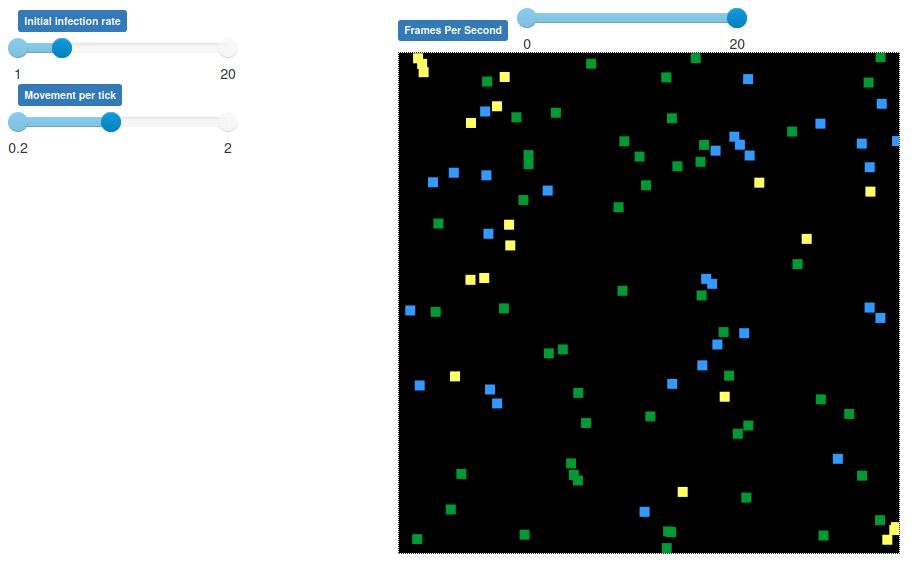
\includegraphics[width=0.75\textwidth]{epidemic_mesa.png}
  \caption{Visuel interface fra \texttt{EpidemicModelRun.py}.}
\end{figure}
\section{Konklusion}

\end{document}
